\subsection{Diagrama de Voronoi}

Segundo \citeonline{rodrigues_diagrama_2019} diagrama de Voronoi é o particionamento do espaço onde cada região é associada a um ponto do conjunto.

O diagrama de Voronoi é gerado a partir das distancias euclidianas entre os vizinhos de um conjunto de pontos do plano\space
\cite{diagrama_de_voronoi:_uma_exploracao_nas_distancias_euclidiana_e_do_taxi}. Esse diagrama possui uma gama de utilizações, por exemplo, estudar epidemias, encontrar o 
ponto mais próximo, calcular a precipitação de uma área, estudar os padrões de crescimento das florestas, etc,\space\cite{poligonos_de_thiessen_ou_voronoi}. 

Seja um conjunto de índices $I_n = \{1, 2, 3, ..., n\}$ e $A = \{p_1, p_2, ..., p_n\} \subset \mathbb{R}^2$ um conjunto de pontos onde $2 \leq n < \infty$, definimos como região de Voronoi o conjunto de pontos associado a $p_i$, onde d é a distancia euclidiana

\begin{equation}
	V(p_i) = \{p|d(p_i,p) \leq d(p_i,p);i \neq j, i, j \in I_n\},
\end{equation}


temos o conjunto formado por essas regiões sendo $V(A) = {V(1), V(2), V(3), ..., V(n)}$ \cite{rodrigues_diagrama_2019}.

Na figura \cref{fig:diagrama_voronoi} podemos ver a relação do conjuntos de pontos com o diagrama de Voronoi.

\begin{figure}[H]
	\centering
	\caption{Diagrama de Voronoi.}
	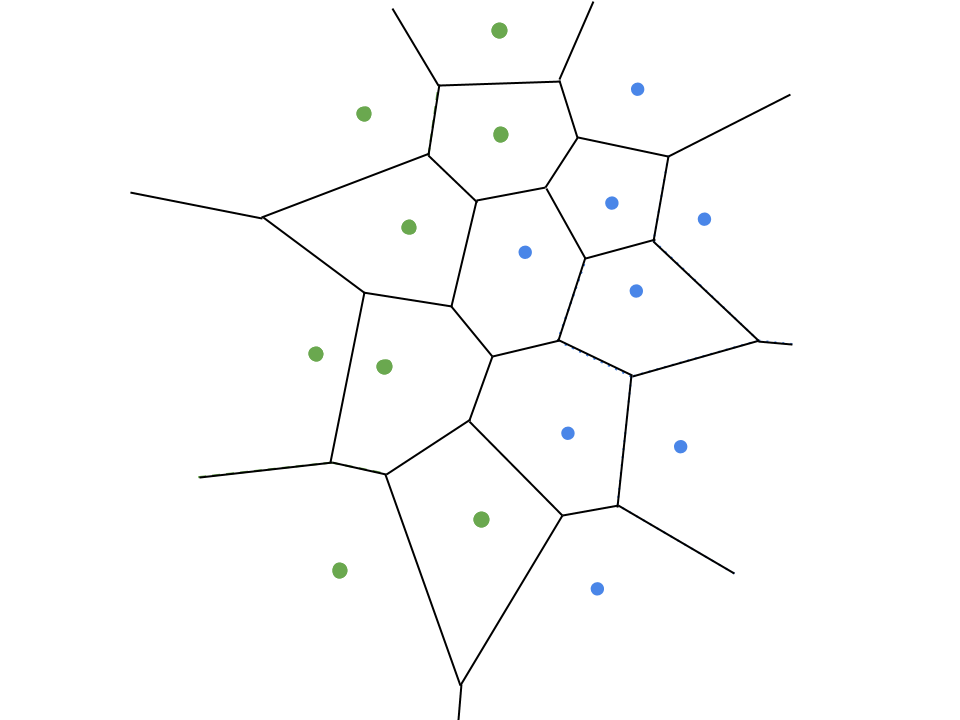
\includegraphics[width=0.6\textwidth]{figures/diagrama_de_voronoi.png}
	\legend{Fonte: \citeonline{thomazthz_diagrama_2014}}
	\label{fig:diagrama_voronoi}
\end{figure}
